\documentclass[10pt,a4paper]{article}
\usepackage[utf8]{inputenc}
\usepackage[french]{babel}
\usepackage[T1]{fontenc}
\usepackage{amsmath}
\usepackage{amsfonts}
\usepackage{amssymb}
\usepackage{makeidx}
\usepackage{xcolor} 
\usepackage{graphicx}
\usepackage{lmodern}
\usepackage[many]{tcolorbox}
\usetikzlibrary{shadows}
\usepackage{kpfonts}
\usepackage{geometry}
\usepackage{xcolor} 
\usepackage{fancybox}
\usepackage{graphicx}
\usepackage{lmodern}
\author{KOUTEMA Ditoma}

\begin{document}
\newtcolorbox{shadedbox}{
  drop shadow southeast,
  breakable,
  enhanced jigsaw,
  colback=white,
}

\begin{shadedbox}
\begin{center}
\huge \textcolor{blue}{RAPPORT DU TP SUR LE FRAMEWORK DJANGO}
\end{center}
\end{shadedbox}
%fin box%
\large{\begin{center}
fait par : 
\end{center}}
\begin{center}
\huge{KOUTEMA Ditoma}
\end{center}
\newpage
\tableofcontents
\newpage

\section{ALiaons Python3 !}
\begin{enumerate}
\item Un alias est un adverbe qui permet de donner un surnom a une variable ou un objet en python
\item La différence après avoir lancé python et python3 est que :\\
\begin{itemize}

\item Quand on lance \textcolor{blue}{python}, on remarque que la commande python n'a pas été trouvée c'est à dire cette commande n'est pas reconnue.
\item Quand on lance \textcolor{blue}{python3},on remarque que la commande est reconnue et nous affiche python et sa version. Donc python3 donne \textcolor{blue}{Python 3.10.12}.\\
\begin{center}
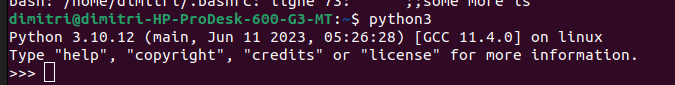
\includegraphics[scale=0.5]{1.png}\\
\end{center}
\item Version de python installer est \textcolor{blue}{3.10.12} après avoir fixer mon alias en \textcolor{blue}{py}
\begin{verbatim}
dimitri@dimitri-HP-ProDesk-600-G3-MT:~$ py
Python 3.10.12 (main, Jun 11 2023, 05:26:28) [GCC 11.4.0] on linux
Type "help", "copyright", "credits" or "license" for more information.
>>> 
\end{verbatim}
\end{itemize}
\end{enumerate}

\section{Installation pip }
\begin{enumerate}
\item
\begin{itemize}
\item[]
\item[•] pip est un gestionnaire de paquets utilisé pour installer et gérer des paquets écrits en Python.
\item[•] Les différentes façons d'installer \textcolor{blue}{pip}.\\ Il existe deux mécanismes d'installation de pip tels que : \textcolor{blue}{ensurepip} et \textcolor{blue}{get-pip.py}.
\item[•] Installation via le gestionnaire de paquets de ubuntu \textcolor{blue}{sudo apt-get install python3-pip}.
\end{itemize}
\item
\begin{itemize}
\item[]
\item[•]Installation via téléchargement d'un fichier depuis Internet plutôt que les paquets d'Ubuntu
\end{itemize}

\item
\begin{itemize}
\item[]
\item[•]Commande lancée : \textcolor{blue}{py get-pip.py}
\item[•]J'ai une erreur concernant la version trouvée\\

\begin{center}
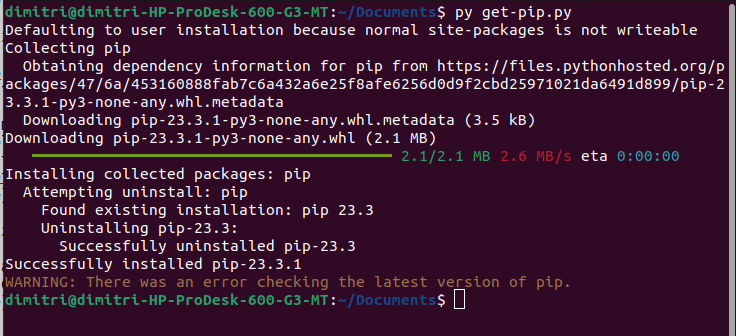
\includegraphics[scale=0.5]{2.png}\\
\end{center}
\end{itemize}

\item
\begin{itemize}
\item[]
\item[•]Installation avec la solution trouvée.
\item[•] Pour résoudre le problème alors export le path :\\ \textcolor{blue}{export PATH=\$PATH:/home/ubuntu/.local/bin}.\\Puis lancer 
\textcolor{blue}{py get-pip.py}\\\\
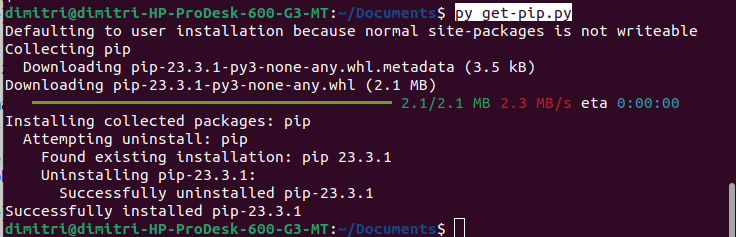
\includegraphics[scale=0.4]{3.png}
\end{itemize}

\item
\begin{itemize}
\item[•] La commande pip --version renvoie : \\\\
\textcolor{blue}{pip 23..1}
%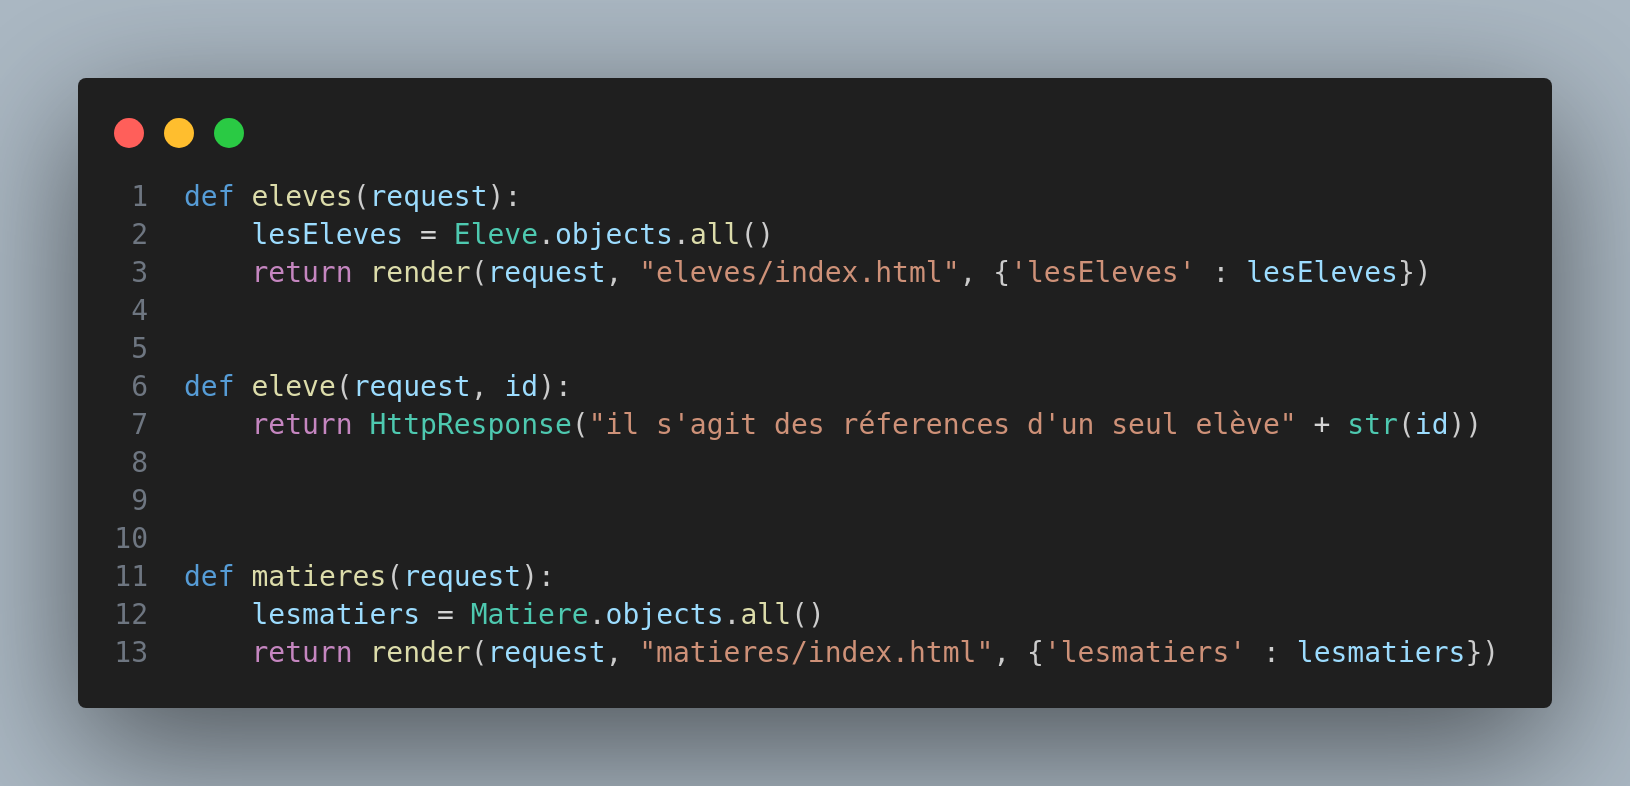
\includegraphics[scale=0.4]{4.png}
\end{itemize}

\end{enumerate}

\section{Créons un environnement virtuel }
\begin{enumerate}
\item
\begin{itemize}
\item[]
\item[•]Un environnement virtuel est un environnement d'exécution isolé. 
\item[•]Il permet d'isoler les paquets utilisés pour un projet, afin d'avoir des versions différentes pour chaque projet.
\item[•] On a besoin parce que le framework django se base sur l'environnement virtuel
\end{itemize}

\item Installation de virtualenv \textcolor{blue}{pip install pipenv} version pipenv, version 2023.10.20
\item Pendant la création, on a deux dossiers qui se sont installé \textcolor{blue}{bin  lib} et un fichier \textcolor{blue}{pyvenv.cfg} qui s'est crée aussi


\item
\begin{itemize}
\item[]
\item Pour créer j'ai fais \textcolor{blue}{virtualenv ap}
\item Pour activer j'ai fais \textcolor{blue}{source nom\_du\_projet/bin/activate}
\item Prefix ajouté (projetnotes) il s'agit du nom de mon projet
\end{itemize}
\item Version de pip maintenant \textcolor{blue}{pip 23.2.1}\\
Il se trouve maintenant dans le projet\\
projetnotes/lib/python3.10/site-packages/pip (python 3.10)
\end{enumerate}


\section{Installons maintenant Django dans l'environnement virtuel}
\begin{enumerate}
\item 
\begin{itemize}
\item
\item[•] Django est un framework du language de programmtion Python.
\item[•] Il sert a la conception des applications web.
\end{itemize}
\item Version \textcolor{blue}{4.2.6}
\begin{verbatim}
dimitri@dimitri-HP-ProDesk-600-G3-MT:~$ py
Python 3.10.12 (main, Jun 11 2023, 05:26:28) [GCC 11.4.0] on linux
Type "help", "copyright", "credits" or "license" for more information.
>>> import django
>>> print(django.get_version())
4.2.6
>>> 

\end{verbatim}
\item Pour désactiver l'environnement virtuel on lance la commande :  \textcolor{blue}{deactivate}
\end{enumerate}
\section{Céation du projet et du serveur de développement}

\begin{enumerate}
\item Un projet est un ensemble de réglages et d’applications pour un site Web particulier tandis que Une application est une application Web qui réalise un certains nombre de tâche donné. 
\item Commande pour créer un projet django :\\ \begin{center}
\textcolor{blue}{django-admin startproject nom\_du\_projet}
\end{center}

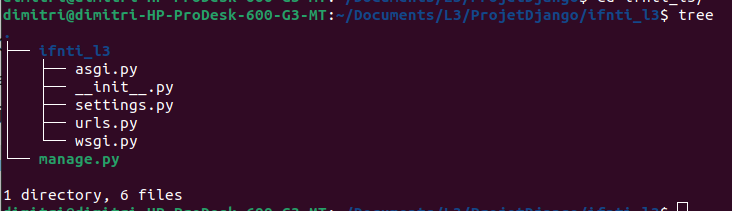
\includegraphics[scale=0.4]{6.png}\\
Le dossier courant contient une architecture qui vient d'être créer.

\item Le fichier \textcolor{red}{manage.py} est le point d'entrée de notre application nouvellement créer.
\item Le fichier \textcolor{red}{settings.py} est le fichier de configuration de notre application.
\item Le fichier \textcolor{red}{\_\_init\_\_.py} permet au dossier qui le contient de pouvoir être traité comme un packet python.
\item Un serve est un environnement qui permet aux développeurs de créer du code et de tester leurs applications. Non.
\item 
\item 
\begin{itemize}
\item[]
\item \textcolor{red}{http} : Hyper Text Transfert Protocol
\item \textcolor{red}{127.0.0.1} : Est l'address local
\item \textcolor{red}{8000} : C'est le port
\end{itemize}
\end{enumerate}

\section{Création de l'application Notes}
\begin{enumerate}
\item Pour quitter le serveur il faut taper la commande : \textcolor{blue}{ctrl + c}
\item La commande pour créer l'application notes faire :\\ \textcolor{blue}{py manage.py startapp notes}. Après avoir lancé cette commande un répertoire \textbf{notes} s'est créer dans le dossier courant
\item Les différents fichiers contenu dans cette application sont : le fichier \textcolor{blue}{manage.py} et le dossier \textcolor{blue}{notes}
\end{enumerate}
\section{Écriture de la première vue}
\begin{enumerate}
\item
\begin{itemize}
\item[]
\item[*] Une vue selon django un exécutable acceptant une requête et renvoyant une réponse.
\item La différence avec le pattern MVC est que le pattern au delà des migrations et contrôleur, intègre la Vue.
\end{itemize}
\item Le fichier \textcolor{blue}{views.py} contient le code \\
Le code va nous retourner la chaîne de caractère Bonjour tout le monde !.
\item Pour créer le fichier urls.py on fait \textcolor{blue}{touch urls.py}
\item Ce code pointe la méthode index qui se trouve dans le fichier views; index est le nom de l'url.
\item le fichier contient le code suivant :\\\\
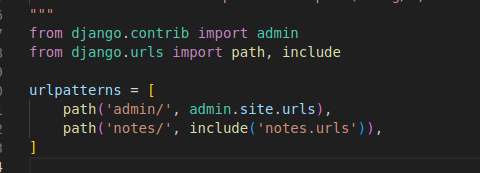
\includegraphics[scale=0.8]{9.png}


%\textit{Contenu du fichier sans commentaire}\\
%\textit{Ce fichier contient un chemin qui contient l'url notes et le fichier urls contenu dans le dossier notes.}

\end{enumerate}












\end{document}